\documentclass[12pt]{article}
\usepackage[utf8]{inputenc}
\usepackage[spanish]{babel}
\usepackage{graphicx}
\usepackage{multicol}
\usepackage{amsmath}

\begin{document}
\textit{Las redes neuronales artificiales y el algoritmo de backpropagation}

%\setlength{\columnsep}{8mm}
%\begin{multicols*}{2}

  Las \textit{redes neuronales artificiales} (en inglés, ANN, Artificial Neural
  Networks) son un modelo simplificado inspirado en el funcionamiento del
  cerebro humano procesar información. Sus aplicaciones principales suelen estar
  relacionadas con tareas como el reconocimiento y clasificación de ciertos
  patrones y esto ha permitido que se puedan crear aplicaciones que van desde el
  detector de spam en los correos electrónicos, traducción automática,
  sugerencias personalizadas en sitios web, hasta la visión por
  computadora.\cite{savage}\\

  Para entender el funcionamiento de las redes neuronales es necesario
  descomponerlo en su unidad mínima, la \textit{neurona}.  El modelo
  de la neurona cuenta con varias entradas multiplicadas por ciertos pesos
  (también conocidos como ponderaciones), están se suman y si la suma es más
  grande que cierto \textit{umbral}, $\theta$ (threshold en inglés), la neurona
  se activa, en caso contrario se encuentra desactivada. De esta manera, las
  entradas se pueden describir mediante la siguiente expresión:

  \[
    u = \sum_{i = 0}^{n} w_ix_i - \theta
  \]

  Por otra parte, la salida de la neurona es generada por una función de
  activación no lineal, la cual usualmente es una función \textit{sigmoide}
  \footnote{Otros modelos como el del perceptrón utiliza la función
  \textit{escalón} como función de activación}, tal y como se muestra a
  continuación:

  \[
    y = f(u) = \dfrac{1}{1+e^{\frac{-u}{T}}}
  \]

  Una representación de gráfica de los conceptos expuesto anteriormente es la
  siguiente:

  %\begin{figure}{ht!}
    %\centering
  \begin{center}
    %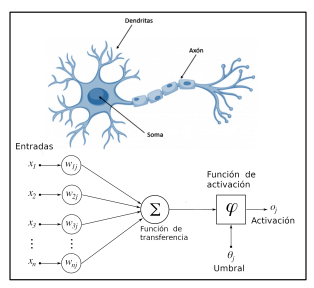
\includegraphics[width=0.7\linewidth]{neurona}
    %\caption{Modelo de una neurona artificial.}
    %\label{fig:neurona}
  \end{center}
  %\end{figure}

  Por lo tanto, al conectar las salidas de una neurona a las entradas de otra se
  forma una red neuronal.

  Las unidades de procesamiento se organizan en capas. Hay tres partes
  normalmente en una red neuronal: una capa de entrada, con unidades que
  representan los campos de entrada, que usualmente se obtiene de los datos
  registrados por sensores para el caso de robots o datasets de imágenes para el
  caso de visión computacional; una o varias capas ocultas; y una capa de
  salida, de acuerdo con \cite[p.~215]{ibm}. La siguiente figura nos permite
  entender el concepto de manera gráfica.

  %\begin{figure}{ht!}
    %\centering
  \begin{center}
    %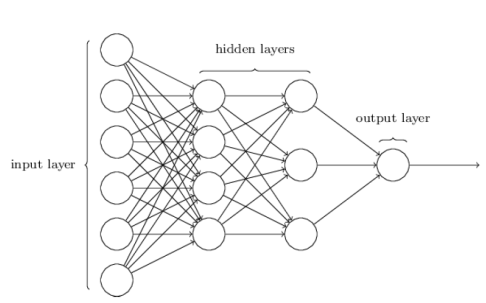
\includegraphics[width=0.7\linewidth]{red-neuronal}
    %\caption{Modelo de una red neuronal artificial.}
    %\label{fig:neurona}
  \end{center}
  %\end{figure}

  El aprendizaje se logra al comparar los valores de entrada multiplicados por
  ciertos pesos que se va ajustando en cada iteración con valores deseados o de
  salida. Este proceso se repite muchas veces con el objetivo de que la red
  mejore sus predicciones hasta haber alzado un criterio de parada o error
  mínimo \cite{savage,ibm}

  Las redes neuronales, al ser parte de los algoritmo de aprendizaje de máquina
  requiere de dos conjuntos de datos pertenecientes a un mismo dataset. El
  primer conjunto es conocido como conjunto de entrenamiento (\textit{training}),
  mientras que el otro es conocido como de prueba (\textit{testing}). La red
  aprende a través del entrenamiento. Continuamente se presentan a la red
  ejemplos para los que se conoce el resultado, y las respuestas que proporciona
  se comparan con los resultados conocidos. La información procedente de esta
  comparación se pasa hacia atrás a través de la red, cambiando los pesos
  gradualmente \cite{minksy}

  \subsection*{Algoritmo de \textit{backpropagation}}

  Para obtener una red neuronal entrenada para cierta tarea se requiere la
  minimización de error cuadrático medio, el cual simplemente esta dado por la
  comparación entre los valores \textit{deseados} y los valores
  \textit{obtenidos} de la red neuronal. Para reducir el error se deben
  encontrar los pesos optimos, por lo cuál se puede utilizar la siguiente
  expresión.

  \[
    \dfrac{\partial E_{j}^{L}}{\partial w_{ij}^{L}} = 
    -\sum_{k=1}^{K} \delta_{jk}^{L} z_{ik}^{L-1}
  \]

  De la expresión anterior se entiende que para minimizar el error se obtiene la
  parcial con respecto a los pesos, para cada de una de las muestras $K$. Además
  $\delta_{k}^{L}$ representa el error modulado de la muestra $k$ en la capa
  $L$.  Sin embargo, para la capa $L$ aún no se conocen el error modulado. El
  error modulado solo se conoce para la última capa (capa de salida). Por lo
  cual se debe buscar una manera de propagar dicho error y es ahí donde se
  utiliza el \textbf{algoritmo de backpropagation}.

  Este algoritmo se denomina backpropagation o de propagación inversa debido a
  que el error se propaga de manera inversa al funcionamiento normal de la red,
  de esta forma, el algoritmo encuentra el error en el proceso de aprendizaje
  desde las capas más internas hasta llegar a la entrada; con base en el cálculo
  de este error se actualizan los pesos de cada capa.
  Este algoritmo es un método de aprendizaje que a su vez utiliza otro método de
  aprendizaje llamado \textit{gradiente descendente}, por que la expresión para
  calcula los pesos basados en la iteración anterior se puede escribir como:

  \[
    w_{ij}^{L}(t+1) = w_{ij}^{L}(t) + \eta
    \sum_{k=1}^{K}\delta_{jk}^{L}z_{ik}^{L-1}
  \]

  $w_{ij}^{L}(t+1)$ representan los pesos recalculados para la iteración $t + 1$
  a partir de una iteración previa. De dicha iteración $t$ ya se conocen el
  error modulado así como las salidas $z$ obtenidas. La siguiente figura puede
  ayudar a entender mejor estos conceptos.

  %\begin{figure}{ht!}
    %\centering
  \begin{center}
    %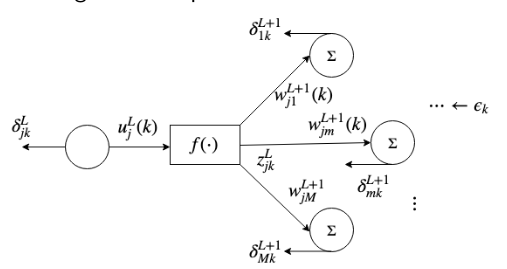
\includegraphics[width=\linewidth]{backpropagation}
    %\caption{Modelo de una red neuronal artificial.}
    %\label{fig:neurona}
  \end{center}
  %\end{figure}

  Finalmente, a la ecuación anterior se le agrega un término para que converja
  más rápido, comparando los valores de los pesos anteriores y agregando ruido
  aleatorio para sacar los pesos de mínimos locales. Por lo que al final la
  expresión para encontrar los pesos aplicando backpropagation es:

  \begin{equation*}
  \begin{split}
    w_{ij}^{L}(t+1) = w_{ij}^{L}(t) + \eta
    \sum_{k=1}^{K}\delta_{jk}^{L}z_{ik}^{L-1} + \\
    \mu[w_{ij}^{L}(t) - w_{ij}^{L}(t-1)] + \epsilon_{ij}^{L}(t)
  \end{split}
  \end{equation*}


  \begin{thebibliography}{9}
    \addtolength{\leftmargin}{0.8in}
    \setlength{\itemindent}{-0.4in}
    \bibitem{savage} 
      Savage, Jesús. \textit{Redes neuronales} en 
      \texttt{https://biorobotics.fi-p.unam.mx/\\wp-content/uploads/Courses/\\
      reconocimiento\_de\_patrones/2021-2/\\lecciones/%
      leccion12\_reconocimiento\\\_de\_patrones\_2021-2.pdf}
    \bibitem{ibm}
      IBM. \textit{El modelo de redes  neuronales} en 
      \texttt{https://www.ibm.com/docs/es/spss-modeler/\\
      SaaS?topic=networks-neural-model}
    \bibitem{ref01} This is reference from Minksy
    \bibitem{ref02} This is reference from Minksy

  \end{thebibliography}

%\end{multicols*}

\end{document}
